\chapter{Modélisation}
\section{Mise sous forme d'espace d'état}
\textit{Écriture des modèles sous forme d'espace d'état}

Notre modélisation sera basée sur les modèles physiques qui décrivent les différents constituants de notre système de procédé : deux moteurs couplés l'un à l'autre par un arbre simple. L'un étant générateur de force mécanique et l'autre générateur de courant afin de faire office de charge (il dissipe son énergie sur une résistance). Il y a aussi un tachymètre couplé à l'arbre principal par un réducteur.
Notre modélisation est donc un modèle de connaissance.

Nous avons choisit de faire une modélisation espace d'état pour différentes raisons. La première est que cette représentation permet de d'étudier facilement la valeur des différents états de façon plus fine (permettant d'étudier la stabilité asymptotique par exemple). Le choix d'un modèle de connaissance améliore aussi l'analyse de l'influence des différents paramètres du modèle. Elle permet de garder les états non observables et non commandables dans le modèle, qu'une modélisation fonction de transfert ne met pas en évidence. Elle permet aussi, pour la suite, de faire un retour d'état aisément, ainsi qu'un observateur. \\ \\

%Notre modèle de connaissance fait apparaitre les 


\begin{figure}[!ht]
\centering
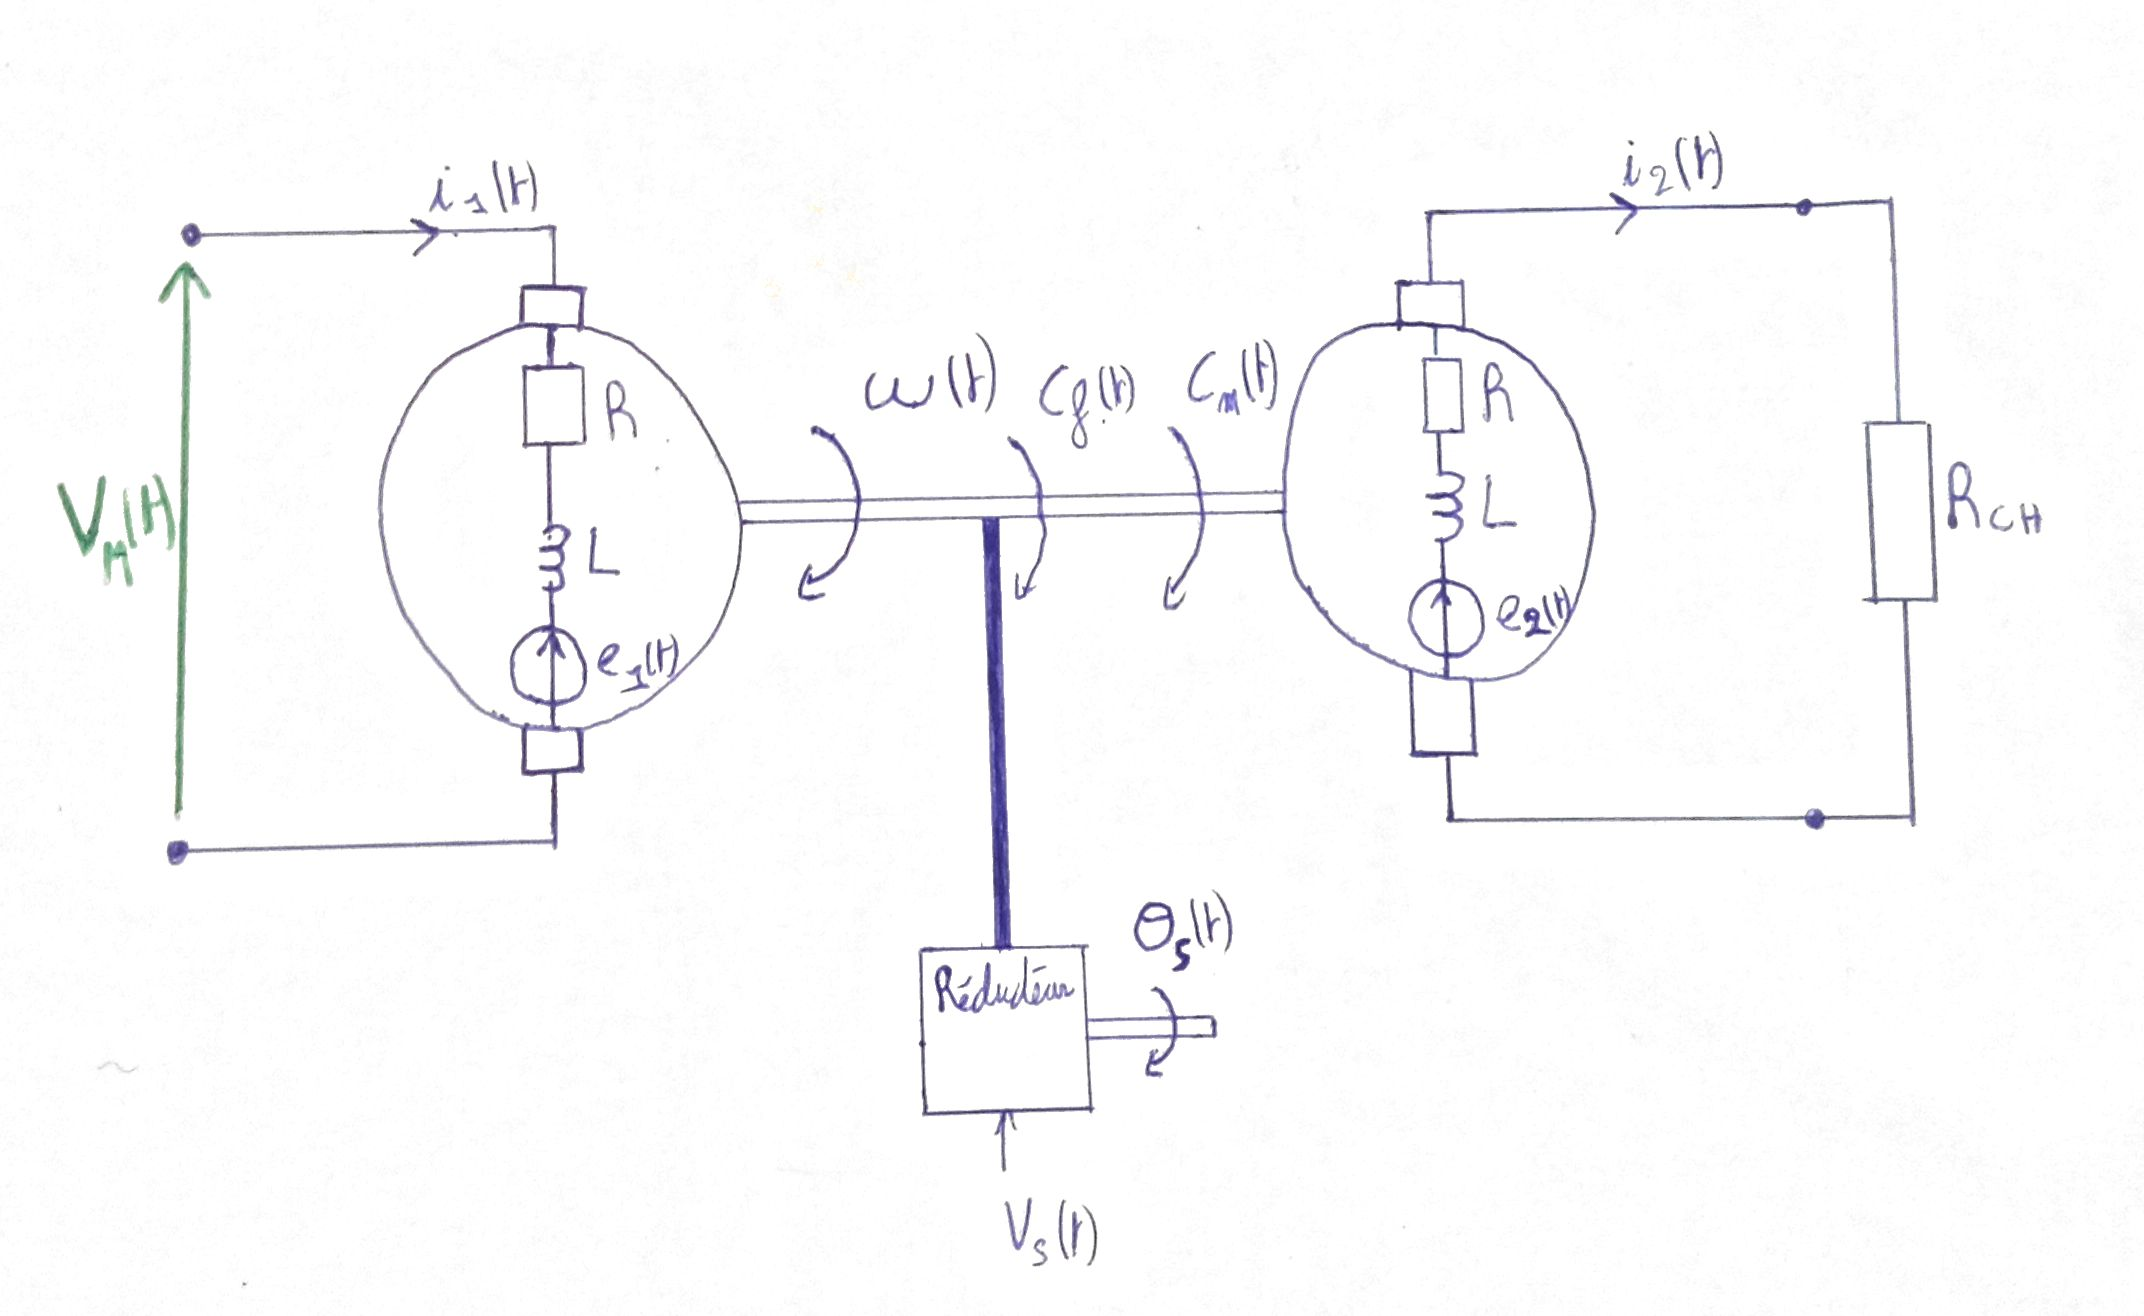
\includegraphics[width=.8\textwidth]{./I/images/schema0.png}
\caption{Schéma électrique/physique du banc moteur}
\label{fig:schema0}
\end{figure}

\hspace{5mm} \textbullet \hspace{5mm} Voici les différentes équations décrivant notre procédé:
\begin{eqnarray}
V_m(t)  					&=& 	R i_1(t) + L \frac{D i_1(t)}{d t} + e_1(t) \\
e_2(t) 						&=& 	(R+R_{CH}) i_2(t) + L \frac{d i_2(t)}{d t} \\
J \frac{d \omega(t)}{dt} 	&=&		C_m(t) + C_f(t)		\\
 \frac{d \theta_s(t)}{dt} 	&=&		\frac{1}{R}\omega(t) \\
\end{eqnarray}

\hspace{5mm} \textbullet \hspace{5mm} Variables d'état :
\begin{equation}
\begin{pmatrix}
\theta_s(t)\\
\omega(t)\\
i_1(t)\\
i_2(t)\\
\end{pmatrix}
=
X(t)
\end{equation}
\subsection{Modèle de niveau 0}
Pour commencer l'étude avec un espace d'état, nous proposons de poser un premier modèle d'état d'ordre 4. Le vecteur d'état choisit est :
\begin{equation}
X(t)=\begin{bmatrix}
i_1\\
i_2\\
\Omega_m\\
\Theta_m\\
\end{bmatrix}
\end{equation} 
Le modèle d'ordre 4 vaut donc :
\begin{align}
\label{EE0}
\left\lbrace
\begin{aligned}
&\dot{X}(t) = \begin{pmatrix}
-\frac{R}{L}	& 	    0				&   -\frac{K_e}{L}	& 0\\
      0			&  -\frac{(R+R_{ch})}{L}	&	-\frac{K_e}{L}	& 0\\
\frac{K_c}{J_2}	&	\frac{K_c}{J_2}		&	\frac{\mu}{J_2}	&	0\\
0&	0&	1&	0
\end{pmatrix}X(t)+\begin{pmatrix}
\frac{1}{L}\\0\\0\\0
\end{pmatrix}V_m(t)\\
&Y(t) = \begin{pmatrix}
0&	0&	K_g	&	0\\
0&	0&	0	&	K_rK_s\\
\end{pmatrix}X(t)
\end{aligned}
\right.
\end{align}
\subsection{Espace d'état d'ordre 2}
Pour correspondre avec un modèle de comportement, nous allons a nouveau réduire la représentation d'état ~\eqref{EE0} pour obtenir un modèle d'ordre 2. Pour cela, nous allons annuler l'effet des dynamiques des courants $i_1$ et $i_2$ qui sont beaucoup plus grandes que les dynamiques de $\omega$ et $\theta$, qui sont celles que nous sommes capable de mesurer et que nous souhaitons asservir.\\

\begin{align}
\label{EE2}
\left\lbrace
\begin{aligned}
&\dot{X}(t) 
=
 \begin{pmatrix}
0 &	1 \\
0	&	-\frac{(K_cK_e)}{J_2R}-\frac{\mu}{J_2}\\
\end{pmatrix}X(t)
+
\begin{pmatrix}
\frac{K_c}{J_2R}\\
0
\end{pmatrix} 
V_m(t)\\
&Y(t) = \begin{pmatrix}
0	&	K_g	\\
K_rK_s	&	0	\\
\end{pmatrix}X(t)
\end{aligned}
\right.
\end{align}

\section{Commande du système EE2}
\subsection{Rédaction du cahier des charges et démarche de réponse}
Après l'étude que nous venons de réaliser sur notre système, nous allons ici exprimé les attentes que doit réaliser la commande que nous allons implémenter. Nous souhaitons avoir : \begin{itemize} 
\item Erreur de position nulle.
\end{itemize}
Pour respecter, nous allons réaliser un placement de valeurs propres par retour d'état.
\subsection{Observateur ordre plein sur EE2}
Pour pouvoir réaliser notre commande par retour d'état, nous devons tous d'abord reconstruire l'ensemble des états du système dont nous n'avons pas accès. Dans notre cas, nous disposons d'une mesure de la vitesse $\Omega$ avec la tension de sortie $V_s$ mais aucune information sur la position $\Theta$, l'implémentation d'un observateur est donc nécessaire pour au minimum reconstruire cet état.\\
Nous préférons reconstruire $\Omega$ et $\theta$ à partir de $V_s$ et de l'entrée de EE2 pour simplifier les calculs nécessaire à sa construction. Il est représenté par :
\begin{align*}
\left\lbrace
\begin{aligned}
&\dot z (t) = Fz(t) + Gy(t) + Hu(t)\\
&\hat x = Mz(t) + Ny(t)\\
&\epsilon = x-\hat{x}
\end{aligned}
\right.
\end{align*} où $x$ représente l'état du système et $\hat{x}$ l'état du système reconstruit.

\section{Adaptation de l'état de EE1}
On a réorganisé les états de EE1 de façon a ce que les état observable soient en haut et les non observable en bas.

\noindent\textbullet\hspace{2mm} Etats observables : $\Omega_m$ et $ \Theta_m$.

\noindent\textbullet\hspace{2mm} Etat non observable : $i_1$

\noindent\textbullet\hspace{2mm} L'espace d'état est donc : 
\begin{equation}
\overline{X} = \begin{bmatrix}
\Omega_m\\
\Theta_m\\
i_1\\
\end{bmatrix}
\end{equation}

Pour passer de $X$ à $\overline{X}$, il faut faire une matrice de passage $P_X$.

 \begin{eqnarray}
 P_X &/&  \overline{X} =P_X \cdot X \\
 P_X &=&\begin{bmatrix}
 0 & 0 & 1 \\
 1 & 0 & 0 \\
 0 & 1 & 0 \\
\end{bmatrix}  \\
 \end{eqnarray}

Maintenant, nous devons calculer $\overline{A}$, $\overline{B}$, $\overline{C}$, $\overline{D}$ pour le nouvel espace d'état lié à $\overline{X}$.

\begin{equation}%
	\left\lbrace%
	\begin{matrix}
		\overline{A} &=& P^{-1} A P \\%
		\overline{B} &=& P^{-1} B \\%
		\overline{C} &=& C P%	
	\end{matrix}
\right.%
\end{equation}
